\section{Where We Left Off}


\begin{frame}{Tests So Far}
    \begin{itemize}
        \item Overall significance: $H_0:\beta_1=\cdots=\beta_k=0$ with $F_0=\MSR/\MSRes$.
        \item Individual coefficient: $H_0:\beta_j=0$ with $t_0=\hat\beta_j/\se(\hat\beta_j)$.
        \item Group of terms (Lecture 8): partial $F$-test comparing a full and a reduced model.
        \item Delivery time data, $n=25$, $x_1$ = number of cases, $x_2$ = distance (ft): $\hat y = 2.341 + 1.616\,x_1 + 0.0144\,x_2$, $R^2 = 0.9596$.
        \item Overall test: $F_0=261.24$ on $(2,22)$ degrees of freedom. Distance: $t_0=3.98$, $p=0.0006$.
    \end{itemize}
\end{frame}


\begin{frame}{Beyond One Coefficient at a Time}
    Questions that a single $t$-test or the overall $F$-test cannot answer:
    \svspace{0.5em}
    \begin{itemize}
        \item Does a \emph{group} of regressors improve the fit once the others are already in the model?
        \item Do two regressors have the same effect, $\beta_j=\beta_k$?
        \item Is a coefficient, or a combination of coefficients, equal to a specified value?
    \end{itemize}
    \svspace{0.5em}
    All three are answered by comparing a \emph{reduced} model with a \emph{full} model. Lecture 8 used this comparison to test dummy variables and interactions; this lecture explains why the test works and extends it to all three questions.
\end{frame}


\section{Reduced vs. Full Model}


\begin{frame}{Partitioning the Coefficient Vector}
    Model with $p$ parameters ($k=p-1$ regressors):
    \[
    \by = \bX\bbeta + \bvarepsilon
    \]
    Split $\bbeta$ and the columns of $\bX$ into two blocks:
    \[
    \bbeta =
    \begin{bmatrix}
        \bbeta_{(1)} \\ \bbeta_{(2)}
    \end{bmatrix},
    \qquad
    \bX = \begin{bmatrix} \bX_1 & \bX_2 \end{bmatrix}
    \]
    \begin{itemize}
        \item $\bbeta_{(1)}$ is $(p-q)\times 1$ and contains the intercept.
        \item $\bbeta_{(2)}$ is $q\times 1$: the $q$ coefficients under test.
    \end{itemize}
\end{frame}


\begin{frame}{The Full Model}
    \[
    \by = \bX\bbeta + \bvarepsilon = \bX_1\bbeta_{(1)} + \bX_2\bbeta_{(2)} + \bvarepsilon
    \]
    \begin{itemize}
        \item Uses all $p$ parameters.
        \item Least-squares fit: $\hat{\bbeta} = (\bX'\bX)^{-1}\bX'\by$.
        \item Residual sum of squares $\SSRes(\FM)$ with $n-p$ degrees of freedom.
        \item Error variance estimate: $\MSRes = \SSRes(\FM)/(n-p)$.
    \end{itemize}
\end{frame}


\begin{frame}{The Hypothesis and the Reduced Model}
    \[
    H_0:\bbeta_{(2)}=\mathbf{0}
    \qquad\text{versus}\qquad
    H_1:\bbeta_{(2)}\neq\mathbf{0}
    \]
    If $H_0$ is true, the regressors in $\bX_2$ drop out. The \emph{reduced model} is
    \[
    \by = \bX_1\bbeta_{(1)} + \bvarepsilon
    \]
    \begin{itemize}
        \item Least-squares fit: $\hat{\bbeta}_{(1)}=(\bX_1'\bX_1)^{-1}\bX_1'\by$.
        \item Residual sum of squares $\SSRes(\RM)$ with $n-p+q$ degrees of freedom.
    \end{itemize}
\end{frame}


\begin{frame}{Nested Models}
    \begin{itemize}
        \item The reduced model is the full model with $\bbeta_{(2)}$ forced to $\mathbf{0}$.
        \item Every fit the reduced model can produce is also available to the full model.
        \item The full model can only match or improve on the reduced model's fit.
    \end{itemize}
    \[
    \SSRes(\RM) \;\ge\; \SSRes(\FM)
    \]
    The question is whether the improvement is larger than chance alone would produce.
\end{frame}


\begin{frame}{Question: Why Not Just Compare the Residual Sums of Squares?}
    The full model always has the smaller (or equal) residual sum of squares.
    \svspace{0.5em}
    \begin{itemize}
        \item So can we conclude that $\bX_2$ matters whenever $\SSRes(\FM)<\SSRes(\RM)$?
        \item What would a useful comparison need?
    \end{itemize}
    % Answer:
    % - No. Adding even a pure-noise regressor lowers SSRes, so the difference is positive by construction.
    % - The comparison must be scaled by the noise level (MSRes) and by the number of parameters added (q).
    % - That is exactly what the partial F statistic does.
\end{frame}


\begin{frame}{Geometry of Nested Models}
    \begin{columns}[T]
        \begin{column}{0.4\textwidth}
            \begin{itemize}
                \item $\col(\bX_1)\subset\col(\bX)$.
                \item $\hat{\by}_1=\mathbf{H}_1\by$ projects onto the smaller space, $\hat{\by}=\mathbf{H}\by$ onto the larger. Here $\mathbf{H}_1=\bX_1(\bX_1'\bX_1)^{-1}\bX_1'$ is the hat matrix of the reduced model.
                \item $\hat{\by}-\hat{\by}_1$ is the part of the fit due to $\bX_2$.
                \item $\SSRes(\RM)=\|\by-\hat{\by}_1\|^2$ and $\SSRes(\FM)=\|\by-\hat{\by}\|^2$.
            \end{itemize}
        \end{column}
        \begin{column}{0.6\textwidth}
            \centering
            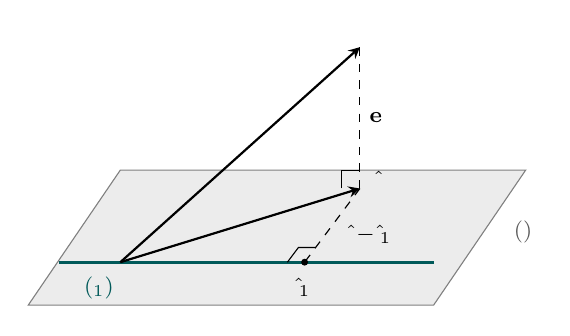
\begin{tikzpicture}[scale=0.78, >=stealth, every node/.style={font=\footnotesize}]
                \fill[gray!15] (0,0)--(6.6,0)--(8.1,2.2)--(1.5,2.2)--cycle;
                \draw[gray] (0,0)--(6.6,0)--(8.1,2.2)--(1.5,2.2)--cycle;
                \node[gray!70!black, anchor=west] at (7.75,1.2) {$\col(\bX)$};
                \draw[very thick, teal!70!black] (0.5,0.7)--(6.6,0.7);
                \node[teal!70!black, anchor=north west] at (0.75,0.62) {$\col(\bX_1)$};
                \coordinate (O) at (1.5,0.7);
                \coordinate (P1) at (4.5,0.7);
                \coordinate (P) at (5.4,1.9);
                \coordinate (Y) at (5.4,4.2);
                \draw[->, thick] (O)--(Y) node[above] {$\by$};
                \draw[->, thick] (O)--(P);
                \node[anchor=west] at (5.55,2.05) {$\hat{\by}$};
                \draw[dashed] (Y)--(P) node[midway, right] {$\mathbf{e}$};
                \draw[dashed] (P)--(P1);
                \node[anchor=west] at (5.1,1.15) {$\hat{\by}-\hat{\by}_1$};
                \fill (P1) circle (1.6pt);
                \node[anchor=north] at (4.5,0.6) {$\hat{\by}_1$};
                \draw (P1)++(-0.28,0)--++(0.18,0.24)--++(0.28,0);
                \draw (P)++(-0.3,0)--++(0,0.3)--++(0.3,0);
            \end{tikzpicture}
        \end{column}
    \end{columns}
\end{frame}


\begin{frame}{Delivery Time Data: Full vs. Reduced Model}
    Test whether distance ($x_2$) adds anything once cases ($x_1$) are in the model.
    \svspace{0.5em}
    \begin{center}
        \small
        \begin{tabular}{llrr}
            \toprule
            Model & Fitted equation & $\SSRes$ & df \\
            \midrule
            Full & $\hat y = 2.341 + 1.616\,x_1 + 0.0144\,x_2$ & 233.73 & 22 \\
            Reduced & $\hat y = 3.321 + 2.176\,x_1$ & 402.13 & 23 \\
            \bottomrule
        \end{tabular}
    \end{center}
    \begin{itemize}
        \item Here $\bbeta_{(1)}=(\beta_0,\beta_1)'$ and $\bbeta_{(2)}=\beta_2$, so $q=1$.
        \item $\MSRes(\FM) = 233.73/22 = 10.62$.
    \end{itemize}
\end{frame}


\section{Extra Sum of Squares}


\begin{frame}{Extra Sum of Squares: Definition}
    Regression sum of squares of the full model, $\SSR(\bbeta)$ with $p-1$ df, and of the reduced model, $\SSR(\bbeta_{(1)})$ with $p-q-1$ df. The \emph{extra sum of squares} due to $\bbeta_{(2)}$ given $\bbeta_{(1)}$ is
    \begin{align}
        \SSR(\bbeta_{(2)}\mid\bbeta_{(1)}) = \SSR(\bbeta) - \SSR(\bbeta_{(1)})
        \label{eq:extra-ss}
    \end{align}
    with $q$ degrees of freedom.
    \svspace{0.5em}

    % Note: here $\SSR=\SST-\SSRes$ is corrected for the mean. MPV uses the uncorrected version, with one more df; the extra sum of squares is the same either way.
\end{frame}


\begin{frame}{Interpreting the Extra Sum of Squares}
    \begin{itemize}
        \item It is the increase in the regression sum of squares when $\bX_2$ is added to a model that already contains $\bX_1$.
        \item The word ``given'' matters: the contribution of $\bX_2$ depends on what is already in the model.
        \item Equivalently, it is how much of the unexplained variation $\bX_2$ removes.
    \end{itemize}
\end{frame}


\begin{frame}{Extra Sum of Squares as a Reduction in $\SSRes$}
    Both models decompose the same total sum of squares:
    \begin{align*}
        \SST &= \SSR(\bbeta) + \SSRes(\FM) \\
        \SST &= \SSR(\bbeta_{(1)}) + \SSRes(\RM)
    \end{align*}
    Subtracting the second line from the first and using \eqref{eq:extra-ss}:
    \begin{align}
        \SSR(\bbeta_{(2)}\mid\bbeta_{(1)}) = \SSRes(\RM) - \SSRes(\FM)
        \label{eq:extra-ss-res}
    \end{align}
\end{frame}


\begin{frame}{Partitioning the Regression Sum of Squares}
    Rearranging \eqref{eq:extra-ss}:
    \[
    \SSR(\bbeta) = \SSR(\bbeta_{(1)}) + \SSR(\bbeta_{(2)}\mid\bbeta_{(1)})
    \]
    \begin{itemize}
        \item The regression sum of squares splits into what $\bX_1$ explains and what $\bX_2$ adds.
        \item Degrees of freedom split the same way: $p-1=(p-q-1)+q$.
    \end{itemize}
\end{frame}


\begin{frame}{Delivery Time Data: Extra Sum of Squares for Distance}
    \begin{align*}
        \SSR(\beta_2\mid\beta_1,\beta_0) &= \SSR(\bbeta) - \SSR(\bbeta_{(1)}) = 5550.81 - 5382.41 = 168.40 \\
        &= \SSRes(\RM) - \SSRes(\FM) = 402.13 - 233.73 = 168.40
    \end{align*}
    \begin{itemize}
        \item Both routes agree, as \eqref{eq:extra-ss-res} requires.
        \item Adding distance to a model with cases reduces the residual sum of squares by 168.40, from 402.13 to 233.73.
    \end{itemize}
\end{frame}


\begin{frame}{Distribution Under $H_0$}
    Assume $\bvarepsilon\sim N(\mathbf{0},\sigma^2\mathbf{I})$. If $H_0:\bbeta_{(2)}=\mathbf{0}$ is true:
    \begin{itemize}
        \item $\SSR(\bbeta_{(2)}\mid\bbeta_{(1)})/\sigma^2\sim\chi^2_q$.
        \item $\SSRes(\FM)/\sigma^2\sim\chi^2_{n-p}$.
        \item The two are independent.
    \end{itemize}
    \svspace{0.5em}
    The next frames show why, using the hat matrices of the two models.
\end{frame}


\begin{frame}{Projection Form of the Extra Sum of Squares}
    Hat matrices of the full and reduced models:
    \[
    \mathbf{H}=\bX(\bX'\bX)^{-1}\bX',
    \qquad
    \mathbf{H}_1=\bX_1(\bX_1'\bX_1)^{-1}\bX_1'
    \]
    Residual sums of squares are quadratic forms in $\by$:
    \begin{align*}
        \SSRes(\FM) &= \by'(\mathbf{I}-\mathbf{H})\by \\
        \SSRes(\RM) &= \by'(\mathbf{I}-\mathbf{H}_1)\by \\
        \SSR(\bbeta_{(2)}\mid\bbeta_{(1)}) &= \by'(\mathbf{H}-\mathbf{H}_1)\by
    \end{align*}
\end{frame}


\begin{frame}{Why $\mathbf{H}-\mathbf{H}_1$ Is a Projection: Step 1}
    $\col(\bX_1)\subset\col(\bX)$, so projecting a vector already in $\col(\bX_1)$ onto $\col(\bX)$ leaves it unchanged: $\mathbf{H}\bX_1=\bX_1$. Hence
    \begin{align*}
        \mathbf{H}\mathbf{H}_1 &= \mathbf{H}\bX_1(\bX_1'\bX_1)^{-1}\bX_1' = \bX_1(\bX_1'\bX_1)^{-1}\bX_1' = \mathbf{H}_1 \\
        \mathbf{H}_1\mathbf{H} &= (\mathbf{H}\mathbf{H}_1)' = \mathbf{H}_1
    \end{align*}
\end{frame}


\begin{frame}{Why $\mathbf{H}-\mathbf{H}_1$ Is a Projection: Step 2}
    \begin{align*}
        (\mathbf{H}-\mathbf{H}_1)^2 &= \mathbf{H} - \mathbf{H}\mathbf{H}_1 - \mathbf{H}_1\mathbf{H} + \mathbf{H}_1 = \mathbf{H}-\mathbf{H}_1 \\
        \rank(\mathbf{H}-\mathbf{H}_1) &= \tr(\mathbf{H}-\mathbf{H}_1) = p-(p-q) = q
    \end{align*}
    \begin{itemize}
        \item $\mathbf{H}-\mathbf{H}_1$ is symmetric and idempotent of rank $q$: a projection onto a $q$-dimensional space.
        \item Also $(\mathbf{H}-\mathbf{H}_1)(\mathbf{I}-\mathbf{H})=\mathbf{0}$, so the two quadratic forms involve orthogonal pieces of $\by$ and are independent.
        \item Under $H_0$, $\E[\by]=\bX_1\bbeta_{(1)}$ is annihilated (sent to $\mathbf{0}$) by $\mathbf{H}-\mathbf{H}_1$, so the form depends on $\bvarepsilon$ only and is $\sigma^2\chi^2_q$.
    \end{itemize}
\end{frame}


\begin{frame}{Background: What Does ``Annihilate'' Mean?}
    A matrix $\mathbf{A}$ \emph{annihilates} a vector $\mathbf{v}$ if
    \[
        \mathbf{A}\mathbf{v}=\mathbf{0}
    \]
    \begin{itemize}
        \item Nothing of $\mathbf{v}$ survives the multiplication.
        \item The set of all vectors that $\mathbf{A}$ annihilates is its \emph{null space}.
        \item Familiar case: $\mathbf{I}-\mathbf{H}$ annihilates every vector in $\col(\bX)$, since $(\mathbf{I}-\mathbf{H})\bX\bbeta=\bX\bbeta-\bX\bbeta=\mathbf{0}$. This is why the residuals $\mathbf{e}=(\mathbf{I}-\mathbf{H})\by=(\mathbf{I}-\mathbf{H})\bvarepsilon$ contain no trace of $\E[\by]$.
        \item Here: $\mathbf{H}\bX_1=\bX_1=\mathbf{H}_1\bX_1$, so $\mathbf{H}-\mathbf{H}_1$ annihilates $\col(\bX_1)$, which contains $\E[\by]=\bX_1\bbeta_{(1)}$ under $H_0$.
    \end{itemize}
\end{frame}


\begin{frame}{Question: Why Does the Extra Sum of Squares Have $q$ Degrees of Freedom?}
    \begin{itemize}
        \item We added $q$ columns to the model. How does that show up in the projection picture?
    \end{itemize}
    % Answer:
    % - The extra SS is the squared length of (H - H1)y, a projection onto the part of col(X) orthogonal to col(X1).
    % - That space has dimension p - (p - q) = q, one dimension per added (linearly independent) column.
\end{frame}


\section{Partial F-Test}


\begin{frame}{The Partial $F$ Statistic}
    \begin{align}
        F_0 = \frac{\SSR(\bbeta_{(2)}\mid\bbeta_{(1)})/q}{\MSRes}
        \label{eq:partial-F}
    \end{align}
    \begin{itemize}
        \item $\MSRes$ comes from the \emph{full} model. It estimates $\sigma^2$ without bias whether or not $H_0$ is true; the reduced model's $\MSRes$ overestimates $\sigma^2$ when $H_0$ is false, which would shrink $F_0$ exactly when we want to reject.
        \item Under $H_0:\bbeta_{(2)}=\mathbf{0}$, $F_0\sim F_{q,\,n-p}$.
        \item Reject $H_0$ at level $\alpha$ if $F_0>F_{\alpha,\,q,\,n-p}$.
    \end{itemize}
\end{frame}


\begin{frame}{Partial $F$ Statistic from the Residual Sums of Squares}
    Substituting \eqref{eq:extra-ss-res} into \eqref{eq:partial-F}:
    \begin{align}
        F_0 = \frac{\bigl[\SSRes(\RM)-\SSRes(\FM)\bigr]/q}{\SSRes(\FM)/(n-p)}
        \label{eq:partial-F-res}
    \end{align}
    Only the two residual sums of squares and their degrees of freedom are needed.
\end{frame}


\begin{frame}{Reading the Statistic}
    \begin{itemize}
        \item Numerator: the average reduction in $\SSRes$ per added parameter.
        \item Denominator: the noise level $\sigma^2$, estimated from the full model.
        \item $F_0\approx 1$: the added regressors reduce $\SSRes$ no more than noise would.
        \item $F_0$ large: the reduction is too big to be chance, so reject $H_0$.
    \end{itemize}
\end{frame}


\begin{frame}{ANOVA Table with Extra-Sum-of-Squares Rows}
    \begin{center}
        \small
        \begin{tabular}{lcccc}
            \toprule
            Source & SS & df & MS & $F_0$ \\
            \midrule
            Regression & $\SSR(\bbeta)$ & $p-1$ & $\MSR$ & $\MSR/\MSRes$ \\
            \quad $\bbeta_{(1)}$ & $\SSR(\bbeta_{(1)})$ & $p-q-1$ & & \\
            \quad $\bbeta_{(2)}\mid\bbeta_{(1)}$ & $\SSR(\bbeta_{(2)}\mid\bbeta_{(1)})$ & $q$ & $\SSR(\bbeta_{(2)}\mid\bbeta_{(1)})/q$ & $\dfrac{\SSR(\bbeta_{(2)}\mid\bbeta_{(1)})/q}{\MSRes}$ \\
            Residual & $\SSRes$ & $n-p$ & $\MSRes$ & \\
            Total & $\SST$ & $n-1$ & & \\
            \bottomrule
        \end{tabular}
    \end{center}
\end{frame}


\begin{frame}{Special Case: The Overall $F$-Test}
    Take $\bbeta_{(1)}=\beta_0$ and $\bbeta_{(2)}=(\beta_1,\dots,\beta_k)'$, so $q=p-1=k$.
    \begin{itemize}
        \item Reduced model: intercept only, $\hat y_i=\bar y$, so $\SSRes(\RM)=\SST$.
        \item Extra sum of squares: $\SST-\SSRes(\FM)=\SSR(\bbeta)$.
    \end{itemize}
    \[
    F_0 = \frac{\SSR/k}{\MSRes} = \frac{\MSR}{\MSRes}
    \]
    The overall test is the partial $F$-test with every slope in the tested block.
\end{frame}


\begin{frame}{Special Case: One Coefficient}
    Take $q=1$, so $\bbeta_{(2)}=\beta_j$. With $C_{jj}=[(\bX'\bX)^{-1}]_{jj}$:
    \[
    \SSR(\beta_j\mid\text{all other }\beta\text{'s}) = \frac{\hat\beta_j^{\,2}}{C_{jj}}
    \]
    \begin{align*}
        F_0 = \frac{\hat\beta_j^{\,2}/C_{jj}}{\MSRes} = \left(\frac{\hat\beta_j}{\sqrt{\MSRes\,C_{jj}}}\right)^{2} = t_0^2
    \end{align*}
    The partial $F$-test for a single coefficient is the two-sided $t$-test, since $F_{1,\nu}=t_\nu^2$.
    \svspace{0.5em}

    Why $\hat\beta_j^{\,2}/C_{jj}$: this is the matrix form \eqref{eq:ssh} of the general linear hypothesis (later in this lecture) with $\mathbf{T}$ the row that has $1$ in the position of $\beta_j$ and $0$ elsewhere, so $\mathbf{T}\hat{\bbeta}=\hat\beta_j$ and $\mathbf{T}(\bX'\bX)^{-1}\mathbf{T}'=C_{jj}$.
\end{frame}


\begin{frame}{Delivery Time Data: Does Distance Add to Cases?}
    $H_0:\beta_2=0$ versus $H_1:\beta_2\neq0$, given $x_1$ in the model.
    \svspace{0.5em}
    \begin{center}
        \small
        \begin{tabular}{lrr}
            \toprule
            & $\SSRes$ & df \\
            \midrule
            Full: $x_1,x_2$ & 233.73 & 22 \\
            Reduced: $x_1$ & 402.13 & 23 \\
            \midrule
            Difference & 168.40 & 1 \\
            \bottomrule
        \end{tabular}
    \end{center}
\end{frame}


\begin{frame}{Delivery Time Data: Partial $F$ for Distance}
    \begin{align*}
        F_0 = \frac{168.40/1}{233.73/22} = \frac{168.40}{10.62} = 15.85
    \end{align*}
    \begin{itemize}
        \item $F_{0.05,1,22}=4.30$ and $p=0.0006$: reject $H_0$.
        \item Distance contributes significantly given cases.
        \item Check: $t_0=3.98$ for $\beta_2$ and $t_0^2=15.85=F_0$.
    \end{itemize}
\end{frame}


\begin{frame}{Delivery Time Data: Does Cases Add to Distance?}
    Reverse the roles: $H_0:\beta_1=0$, with $x_2$ in the reduced model.
    \begin{align*}
        F_0 = \frac{(1185.39-233.73)/1}{233.73/22} = \frac{951.66}{10.62} = 89.58
    \end{align*}
    \begin{itemize}
        \item $p=3.3\times10^{-9}$: reject $H_0$.
        \item Check: $t_0=9.46$ for $\beta_1$ and $t_0^2=89.58$.
    \end{itemize}
\end{frame}


\begin{frame}{A Second Dataset: Gasoline Mileage}
    MPV Table B.3: 32 automobiles, response $y$ = miles per gallon.
    \svspace{0.5em}
    \begin{itemize}
        \item Regressors used here: horsepower, torque, rear axle ratio, carburetor barrels, weight.
        \item Torque is missing for two cars, so we use the $n=30$ complete cases.
    \end{itemize}
    \[
    y = \beta_0 + \beta_{\mathrm{hp}}x_{\mathrm{hp}} + \beta_{\mathrm{tq}}x_{\mathrm{tq}} + \beta_{\mathrm{ax}}x_{\mathrm{ax}} + \beta_{\mathrm{cb}}x_{\mathrm{cb}} + \beta_{\mathrm{wt}}x_{\mathrm{wt}} + \varepsilon
    \]
    Here $p=6$, so the residual degrees of freedom are $n-p=24$.
\end{frame}


\begin{frame}{Gasoline Mileage: Full Model Fit}
    \begin{center}
        \small
        \begin{tabular}{lrrrr}
            \toprule
            Term & Estimate & Std. error & $t_0$ & $p$-value \\
            \midrule
            Intercept & 29.4244 & 7.0840 & 4.154 & 0.0004 \\
            Horsepower & $-0.0204$ & 0.0714 & $-0.285$ & 0.778 \\
            Torque & $-0.0240$ & 0.0525 & $-0.457$ & 0.652 \\
            Rear axle ratio & 1.9610 & 2.0862 & 0.940 & 0.357 \\
            Carburetor barrels & 0.4261 & 0.9560 & 0.446 & 0.660 \\
            Weight & $-0.00235$ & 0.00192 & $-1.224$ & 0.233 \\
            \bottomrule
        \end{tabular}
    \end{center}
    $\SSR=860.48$ (5 df), $\SSRes=278.62$ (24 df), $\MSRes=11.609$, $R^2=0.755$, overall $F_0=14.82$ ($p\approx10^{-6}$).
\end{frame}


\begin{frame}{Question: Every $t$-Test Is Insignificant, Yet the Overall $F$ Is Large}
    \begin{itemize}
        \item How can the model be highly significant while no individual coefficient is?
        \item Sample correlations: horsepower--torque $0.96$, torque--weight $0.91$, horsepower--weight $0.85$.
    \end{itemize}
    % Answer:
    % - Each t-test measures the contribution of one regressor given all the others.
    % - If the regressors carry overlapping information, removing any one of them costs little because the others cover for it.
    % - The group as a whole still explains a lot, which the overall F (and a partial F on a group) detects.
\end{frame}


\begin{frame}{Gasoline Mileage: Testing a Group of Regressors}
    $H_0:\beta_{\mathrm{hp}}=\beta_{\mathrm{tq}}=\beta_{\mathrm{wt}}=0$, so $q=3$: do the three engine-size and weight measures add anything beyond axle ratio and carburetor?
    \svspace{0.5em}
    \begin{center}
        \small
        \begin{tabular}{lrr}
            \toprule
            & $\SSRes$ & df \\
            \midrule
            Full: hp, tq, ax, cb, wt & 278.62 & 24 \\
            Reduced: ax, cb & 592.96 & 27 \\
            \midrule
            Difference & 314.34 & 3 \\
            \bottomrule
        \end{tabular}
    \end{center}
    Reduced fit: $\hat y = 3.768 + 6.718\,x_{\mathrm{ax}} - 1.713\,x_{\mathrm{cb}}$.
\end{frame}


\begin{frame}{Gasoline Mileage: Partial $F$ Calculation}
    \begin{columns}[T]
        \begin{column}{0.5\textwidth}
            \[
            F_0 = \frac{314.34/3}{278.62/24} = \frac{104.78}{11.609} = 9.03
            \]
            \begin{itemize}
                \item $F_{0.05,3,24}=3.01$.
                \item $p=0.0004$: reject $H_0$.
                \item The group matters even though each member has $p>0.2$ individually.
            \end{itemize}
        \end{column}
        \begin{column}{0.5\textwidth}
            \centering
            % Figure: f_dist_partial.pdf (see extra-ss-gasoline.R)
            \mode<presentation>{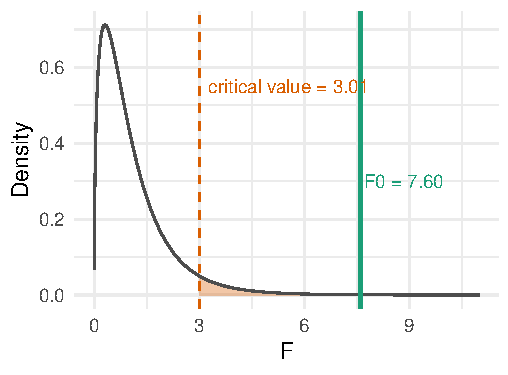
\includegraphics[width=\linewidth]{figures/f_dist_partial.pdf}}
            \mode<article>{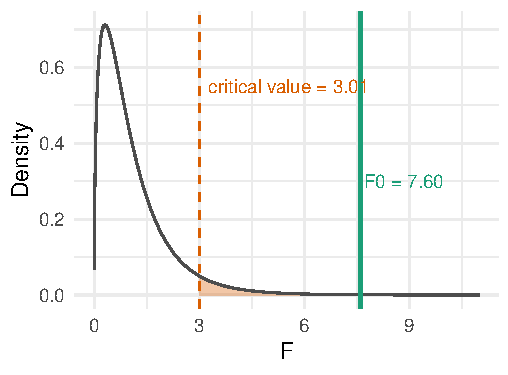
\includegraphics[width=0.8\linewidth]{figures/f_dist_partial.pdf}}
        \end{column}
    \end{columns}
\end{frame}


\begin{frame}{Gasoline Mileage: A Group That Does Not Help}
    $H_0:\beta_{\mathrm{ax}}=\beta_{\mathrm{cb}}=0$, so $q=2$, with hp, tq, wt kept in the model.
    \begin{align*}
        F_0 = \frac{15.03/2}{278.62/24} = \frac{7.514}{11.609} = 0.65
    \end{align*}
    \begin{itemize}
        \item $F_{0.05,2,24}=3.40$ and $p=0.53$: do not reject $H_0$.
        \item Given horsepower, torque and weight, axle ratio and carburetor add nothing detectable.
    \end{itemize}
\end{frame}


\begin{frame}{Question: Why One Partial $F$ Instead of Several $t$-Tests?}
    \begin{itemize}
        \item For $H_0:\beta_{\mathrm{hp}}=\beta_{\mathrm{tq}}=\beta_{\mathrm{wt}}=0$ we could run three $t$-tests. Why is that a poor substitute for $F_0=9.03$?
    \end{itemize}
    % Answer:
    % - Three tests at level alpha give a family-wise error rate above alpha.
    % - The three t statistics are correlated because the regressors are, so they are not separate pieces of evidence.
    % - Here all three t-tests fail to reject (p = 0.78, 0.65, 0.23) while the joint test rejects at p = 0.0004.
    % % (disabled until the joint-ellipse frame in Lecture 5 is restored)
    % % - The joint confidence region is an ellipse, not a box (recall the joint ellipse from Lecture 5).
\end{frame}


\section{General Linear Hypothesis}


\begin{frame}{Linear Restrictions on the Coefficients}
    \[
    H_0:\mathbf{T}\bbeta=\mathbf{0}
    \qquad\text{versus}\qquad
    H_1:\mathbf{T}\bbeta\neq\mathbf{0}
    \]
    \begin{itemize}
        \item $\mathbf{T}$ is a $q\times p$ matrix of rank $q$.
        \item Each row of $\mathbf{T}$ is one linear restriction on $\bbeta$.
        \item Rank $q$ means the $q$ restrictions are independent: none is implied by the others.
    \end{itemize}
\end{frame}


\begin{frame}{Examples of $\mathbf{T}$ for the Gasoline Model}
    Parameter order $(\beta_0,\beta_{\mathrm{hp}},\beta_{\mathrm{tq}},\beta_{\mathrm{ax}},\beta_{\mathrm{cb}},\beta_{\mathrm{wt}})'$.
    \svspace{0.5em}
    \begin{center}
        \small
        \begin{tabular}{lcl}
            \toprule
            Hypothesis & $q$ & $\mathbf{T}$ \\
            \midrule
            $\beta_{\mathrm{wt}}=0$ & 1 & $\begin{bmatrix}0&0&0&0&0&1\end{bmatrix}$ \\[1.2ex]
            $\beta_{\mathrm{hp}}=\beta_{\mathrm{tq}}=0$ & 2 & $\begin{bmatrix}0&1&0&0&0&0\\0&0&1&0&0&0\end{bmatrix}$ \\[2.4ex]
            $\beta_{\mathrm{hp}}=\beta_{\mathrm{tq}}$ & 1 & $\begin{bmatrix}0&1&-1&0&0&0\end{bmatrix}$ \\[1.2ex]
            $\beta_{\mathrm{hp}}=\beta_{\mathrm{tq}},\ \beta_{\mathrm{ax}}=0$ & 2 & $\begin{bmatrix}0&1&-1&0&0&0\\0&0&0&1&0&0\end{bmatrix}$ \\
            \bottomrule
        \end{tabular}
    \end{center}
\end{frame}


\begin{frame}{Subset Tests Are a Special Case}
    If the tested block $\bbeta_{(2)}$ is placed last:
    \[
    \mathbf{T}=\begin{bmatrix}\mathbf{0}_{q\times(p-q)} & \mathbf{I}_q\end{bmatrix}
    \quad\Longrightarrow\quad
    \mathbf{T}\bbeta=\bbeta_{(2)}
    \]
    \begin{itemize}
        \item $H_0:\mathbf{T}\bbeta=\mathbf{0}$ is exactly $H_0:\bbeta_{(2)}=\mathbf{0}$.
        \item Single-coefficient, subset and overall tests are all general linear hypotheses.
        \item The general form also covers restrictions that are not of the form ``coefficients equal zero''.
    \end{itemize}
\end{frame}


\begin{frame}{Obtaining the Reduced Model}
    Impose the restrictions in the full model and simplify.
    \svspace{0.5em}
    Example: $H_0:\beta_{\mathrm{hp}}=\beta_{\mathrm{tq}}=\gamma$. Substituting,
    \[
    y = \beta_0 + \gamma\,(x_{\mathrm{hp}}+x_{\mathrm{tq}}) + \beta_{\mathrm{ax}}x_{\mathrm{ax}} + \beta_{\mathrm{cb}}x_{\mathrm{cb}} + \beta_{\mathrm{wt}}x_{\mathrm{wt}} + \varepsilon
    \]
    \begin{itemize}
        \item The two columns are replaced by their sum.
        \item The reduced model has $p-q=5$ parameters and is fit by ordinary least squares.
    \end{itemize}
\end{frame}


\begin{frame}{Test Statistic for the General Linear Hypothesis}
    \begin{align}
        F_0 = \frac{\bigl[\SSRes(\RM)-\SSRes(\FM)\bigr]/q}{\SSRes(\FM)/(n-p)}
        \label{eq:glh-F}
    \end{align}
    \begin{itemize}
        \item Same form as \eqref{eq:partial-F-res}; $\SSRes(\RM)$ is now the residual sum of squares under the restrictions.
        \item Under $H_0$, $F_0\sim F_{q,\,n-p}$. Reject if $F_0>F_{\alpha,\,q,\,n-p}$.
    \end{itemize}
\end{frame}


\begin{frame}{Matrix Form of the Test}
    The difference in residual sums of squares can be computed from the full-model fit alone:
    \begin{align}
        \SSRes(\RM)-\SSRes(\FM) = \SSH = (\mathbf{T}\hat{\bbeta})'\bigl[\mathbf{T}(\bX'\bX)^{-1}\mathbf{T}'\bigr]^{-1}(\mathbf{T}\hat{\bbeta})
        \label{eq:ssh}
    \end{align}
    \begin{itemize}
        \item $F_0=(\SSH/q)/\MSRes$, the same statistic as \eqref{eq:glh-F}.
        \item No reduced model needs to be fit.
    \end{itemize}
    \svspace{0.5em}
    The next two frames derive \eqref{eq:ssh}.
\end{frame}


\begin{frame}{Deriving $\SSH$, Step 1: Restricted Least Squares}
    The reduced-model fit $\tilde{\bbeta}$ minimizes $(\by-\bX\bbeta)'(\by-\bX\bbeta)$ subject to $\mathbf{T}\bbeta=\mathbf{0}$. With a Lagrange multiplier vector $\boldsymbol{\lambda}$ ($q\times1$), set the derivative of
    \[
    (\by-\bX\bbeta)'(\by-\bX\bbeta) + 2\boldsymbol{\lambda}'\mathbf{T}\bbeta
    \]
    to zero: $\bX'\bX\tilde{\bbeta}=\bX'\by-\mathbf{T}'\boldsymbol{\lambda}$, so $\tilde{\bbeta}=\hat{\bbeta}-(\bX'\bX)^{-1}\mathbf{T}'\boldsymbol{\lambda}$. Imposing $\mathbf{T}\tilde{\bbeta}=\mathbf{0}$ gives $\boldsymbol{\lambda}=\bigl[\mathbf{T}(\bX'\bX)^{-1}\mathbf{T}'\bigr]^{-1}\mathbf{T}\hat{\bbeta}$, hence
    \begin{align}
        \tilde{\bbeta} = \hat{\bbeta} - (\bX'\bX)^{-1}\mathbf{T}'\bigl[\mathbf{T}(\bX'\bX)^{-1}\mathbf{T}'\bigr]^{-1}\mathbf{T}\hat{\bbeta}
        \label{eq:restricted-ls}
    \end{align}
\end{frame}


\begin{frame}{Deriving $\SSH$, Step 2: The Residual Sum of Squares}
    Write the reduced-model residuals as $\by-\bX\tilde{\bbeta}=\mathbf{e}+\bX(\hat{\bbeta}-\tilde{\bbeta})$. The cross term vanishes because $\bX'\mathbf{e}=\mathbf{0}$:
    \[
    \SSRes(\RM) = \mathbf{e}'\mathbf{e} + (\hat{\bbeta}-\tilde{\bbeta})'\bX'\bX(\hat{\bbeta}-\tilde{\bbeta})
    \]
    Let $\mathbf{M}=\mathbf{T}(\bX'\bX)^{-1}\mathbf{T}'$. By \eqref{eq:restricted-ls}, $\hat{\bbeta}-\tilde{\bbeta}=(\bX'\bX)^{-1}\mathbf{T}'\mathbf{M}^{-1}\mathbf{T}\hat{\bbeta}$, so
    \begin{align*}
        \SSRes(\RM)-\SSRes(\FM)
        &= (\mathbf{T}\hat{\bbeta})'\mathbf{M}^{-1}\,\mathbf{T}(\bX'\bX)^{-1}\bX'\bX(\bX'\bX)^{-1}\mathbf{T}'\,\mathbf{M}^{-1}(\mathbf{T}\hat{\bbeta}) \\
        &= (\mathbf{T}\hat{\bbeta})'\mathbf{M}^{-1}\mathbf{M}\mathbf{M}^{-1}(\mathbf{T}\hat{\bbeta}) = (\mathbf{T}\hat{\bbeta})'\mathbf{M}^{-1}(\mathbf{T}\hat{\bbeta}) = \SSH
    \end{align*}
\end{frame}


\begin{frame}{Why the Quadratic Form Works}
    \begin{itemize}
        \item $\Var(\mathbf{T}\hat{\bbeta})=\sigma^2\,\mathbf{T}(\bX'\bX)^{-1}\mathbf{T}'$.
        \item Under $H_0$, $\mathbf{T}\hat{\bbeta}$ has mean $\mathbf{0}$, so $\SSH/\sigma^2$ is a standardized squared length of a $q$-dimensional normal vector: $\chi^2_q$.
        \item $\SSH$ depends on the data only through $\hat{\bbeta}$, and $\hat{\bbeta}$ is independent of $\MSRes$ (Lecture 5). So $F_0=(\SSH/q)/\MSRes\sim F_{q,\,n-p}$ under $H_0$.
        \item For $q=1$, $\SSH/\MSRes$ reduces to $(\mathbf{T}\hat{\bbeta})^2/\bigl(\MSRes\,\mathbf{T}(\bX'\bX)^{-1}\mathbf{T}'\bigr)=t_0^2$.
    \end{itemize}
\end{frame}


\begin{frame}{Gasoline Mileage: $H_0:\beta_{\mathrm{hp}}=\beta_{\mathrm{tq}}$ by the Matrix Form}
    $\mathbf{T}=\begin{bmatrix}0&1&-1&0&0&0\end{bmatrix}$, $q=1$.
    \begin{align*}
        \mathbf{T}\hat{\bbeta} &= \hat\beta_{\mathrm{hp}}-\hat\beta_{\mathrm{tq}} = -0.02039-(-0.02397) = 0.003582 \\
        \mathbf{T}(\bX'\bX)^{-1}\mathbf{T}' &= 0.001217 \\
        \SSH &= \frac{0.003582^2}{0.001217} = 0.0105 \\
        F_0 &= \frac{0.0105/1}{11.609} = 0.0009
    \end{align*}
    $F_{0.05,1,24}=4.26$ and $p=0.976$: do not reject.
\end{frame}


\begin{frame}{Gasoline Mileage: $H_0:\beta_{\mathrm{hp}}=\beta_{\mathrm{tq}}$ by the Reduced Model}
    Fit $y=\beta_0+\gamma(x_{\mathrm{hp}}+x_{\mathrm{tq}})+\beta_{\mathrm{ax}}x_{\mathrm{ax}}+\beta_{\mathrm{cb}}x_{\mathrm{cb}}+\beta_{\mathrm{wt}}x_{\mathrm{wt}}$:
    \begin{align*}
        \hat y &= 29.352 - 0.02248\,(x_{\mathrm{hp}}+x_{\mathrm{tq}}) \\
        &\quad + 1.999\,x_{\mathrm{ax}} + 0.4307\,x_{\mathrm{cb}} - 0.002374\,x_{\mathrm{wt}} \\
        \SSRes(\RM) &= 278.634 \quad(25\ \df)
    \end{align*}
    \begin{itemize}
        \item $\SSRes(\RM)-\SSRes(\FM)=278.634-278.623=0.0105$, matching $\SSH$.
        \item We cannot reject equality, but that is weak evidence \emph{for} it. Horsepower and torque are correlated at $0.96$, so $\hat\beta_{\mathrm{hp}}-\hat\beta_{\mathrm{tq}}=0.0036$ has standard error $\sqrt{11.609\times0.001217}=0.119$ and 95\% interval $(-0.24,\,0.25)$, far wider than either coefficient. The test has little power.
    \end{itemize}
\end{frame}


\begin{frame}{Gasoline Mileage: Two Restrictions at Once}
    $H_0:\beta_{\mathrm{hp}}=\beta_{\mathrm{tq}}$ and $\beta_{\mathrm{ax}}=0$, so $q=2$. The reduced model has three predictor terms:
    \[
    y=\beta_0+\gamma\,(x_{\mathrm{hp}}+x_{\mathrm{tq}})+\beta_{\mathrm{cb}}x_{\mathrm{cb}}+\beta_{\mathrm{wt}}x_{\mathrm{wt}}+\varepsilon
    \]
    \begin{align*}
        \SSRes(\RM) &= 295.24\ (26\ \df) \\
        F_0 &= \frac{(295.24-278.62)/2}{11.609} = \frac{8.308}{11.609} = 0.72
    \end{align*}
    $F_{0.05,2,24}=3.40$ and $p=0.50$: do not reject.
\end{frame}


\begin{frame}{Nonzero Right-Hand Side: $\mathbf{T}\bbeta=\mathbf{c}$}
    \[
    H_0:\mathbf{T}\bbeta=\mathbf{c}
    \qquad\Longrightarrow\qquad
    \SSH=(\mathbf{T}\hat{\bbeta}-\mathbf{c})'\bigl[\mathbf{T}(\bX'\bX)^{-1}\mathbf{T}'\bigr]^{-1}(\mathbf{T}\hat{\bbeta}-\mathbf{c})
    \]
    The derivation is the same as before, with $\mathbf{T}\hat{\bbeta}$ replaced by $\mathbf{T}\hat{\bbeta}-\mathbf{c}$. Reduced model: move the known part to the left-hand side.
    \begin{itemize}
        \item Example: $H_0:\beta_{\mathrm{cb}}=1$. Regress $y-x_{\mathrm{cb}}$ on the other regressors: $\SSRes(\RM)=282.81$.
        \item $F_0=(282.81-278.62)/11.609=0.36$ and $p=0.55$.
        \item Check: $t_0=(0.4261-1)/0.9560=-0.600$ and $t_0^2=0.36$.
    \end{itemize}
\end{frame}


\begin{frame}{Summary of Special Cases}
    \begin{center}
        \small
        \begin{tabular}{llcl}
            \toprule
            Hypothesis & $\mathbf{T}$ rows & $q$ & Reduced model \\
            \midrule
            Single coefficient & one unit row & 1 & Drop the regressor \\
            Subset & $q$ unit rows & $q$ & Drop the subset \\
            All slopes & $k$ unit rows & $k$ & Intercept only \\
            Equal coefficients & $(\dots,1,\dots,-1,\dots)$ & 1 & Sum the two columns \\
            Several restrictions & $q$ independent rows & $q$ & Substitute all restrictions \\
            \bottomrule
        \end{tabular}
    \end{center}
    All use \eqref{eq:glh-F} with $F_{q,\,n-p}$.
\end{frame}


\begin{frame}{Question: Is $\beta_{\mathrm{hp}}=\beta_{\mathrm{tq}}$ Meaningful?}
    \begin{itemize}
        \item Horsepower and torque are on different scales. Is a test of equal coefficients meaningful?
        \item How could the hypothesis be made scale-free?
    \end{itemize}
    % Answer:
    % - A coefficient is the change in y per unit of its own regressor, so equality of raw coefficients compares unlike units unless the units are comparable.
    % - Standardize the regressors first (centre and divide by the standard deviation) and then test equality of the standardized coefficients.
\end{frame}


\section{Sequential vs. Partial Sums of Squares}


\begin{frame}{Sequential Sums of Squares}
    Enter the regressors in a chosen order $x_1,x_2,\dots,x_k$. The sequential sums of squares are
    \[
    \SSR(\beta_1\mid\beta_0),\quad
    \SSR(\beta_2\mid\beta_0,\beta_1),\quad\dots,\quad
    \SSR(\beta_k\mid\beta_0,\dots,\beta_{k-1})
    \]
    \begin{itemize}
        \item Each is an extra sum of squares with $q=1$.
        \item Each regressor is adjusted only for those \emph{entered before it}.
        \item Software often calls these Type I sums of squares.
    \end{itemize}
\end{frame}


\begin{frame}{Sequential Sums of Squares Add Up}
    Applying \eqref{eq:extra-ss} one regressor at a time telescopes:
    \begin{align}
        \SSR(\bbeta) = \sum_{j=1}^{k}\SSR(\beta_j\mid\beta_0,\dots,\beta_{j-1})
        \label{eq:seq-sum}
    \end{align}
    \begin{itemize}
        \item The decomposition accounts for the whole regression sum of squares.
        \item It depends on the order of entry.
    \end{itemize}
\end{frame}


\begin{frame}{Partial Sums of Squares}
    \[
    \SSR(\beta_j\mid\beta_0,\dots,\beta_{j-1},\beta_{j+1},\dots,\beta_k)
    \]
    \begin{itemize}
        \item Each regressor is adjusted for \emph{all} the others, as if it entered last.
        \item Equal to $t_0^2\,\MSRes$ for the individual $t$-test, hence the partial $F$-test with $q=1$.
        \item Software often calls these Type III sums of squares.
        \item In general they do not add up to $\SSR(\bbeta)$.
    \end{itemize}
\end{frame}


\begin{frame}{Delivery Time Data: Sequential vs. Partial}
    \begin{center}
        \small
        \begin{tabular}{lrrr}
            \toprule
            & \multicolumn{2}{c}{Sequential} & Partial \\
            \cmidrule(lr){2-3}
            & $x_1$ first & $x_2$ first & \\
            \midrule
            Cases ($x_1$) & 5382.41 & 951.66 & 951.66 \\
            Distance ($x_2$) & 168.40 & 4599.15 & 168.40 \\
            \midrule
            Sum & 5550.81 & 5550.81 & 1120.06 \\
            \bottomrule
        \end{tabular}
    \end{center}
    \begin{itemize}
        \item Both sequential columns add to $\SSR(\bbeta)=5550.81$; the partial column does not.
        \item The size of each regressor's share depends on the order.
    \end{itemize}
\end{frame}


\begin{frame}{Question: Which Sequential Sum of Squares Equals the Partial One?}
    \begin{itemize}
        \item In the delivery table, which sequential entries coincide with the partial sums of squares?
        \item Why?
    \end{itemize}
    % Answer:
    % - The regressor entered last: SSR(x2 | x1) = 168.40 in the "x1 first" column, SSR(x1 | x2) = 951.66 in the "x2 first" column.
    % - A last-entered regressor is adjusted for every other regressor, which is the definition of the partial sum of squares.
\end{frame}


\begin{frame}{Gasoline Mileage: Sequential vs. Partial}
    \begin{center}
        \small
        \begin{tabular}{lrrr}
            \toprule
            & \multicolumn{2}{c}{Sequential} & Partial \\
            \cmidrule(lr){2-3}
            & hp, tq, ax, cb, wt & wt, cb, ax, tq, hp & \\
            \midrule
            Horsepower & 723.26 & 0.95 & 0.95 \\
            Torque & 107.17 & 18.71 & 2.42 \\
            Rear axle ratio & 2.78 & 56.81 & 10.26 \\
            Carburetor & 9.87 & 4.71 & 2.31 \\
            Weight & 17.39 & 779.31 & 17.39 \\
            \midrule
            Sum & 860.48 & 860.48 & 33.32 \\
            \bottomrule
        \end{tabular}
    \end{center}
    Horsepower carries 723 when entered first and 0.95 when entered last: the regressors overlap heavily.
\end{frame}


\begin{frame}{When Sequential Equals Partial: Orthogonal Columns}
    If $\bX_1'\bX_2=\mathbf{0}$, then $\SSR(\bbeta_{(2)}\mid\bbeta_{(1)})=\SSR(\bbeta_{(2)})$: the contribution of each block is unaffected by the other, in any order. Here $\SSR(\bbeta_{(2)})$ is the regression sum of squares when $y$ is regressed on $\bX_2$ alone (plus an intercept). Since $\bX_1$ contains the column of ones, $\bX_1'\bX_2=\mathbf{0}$ also requires every column of $\bX_2$ to have mean zero.
    \begin{itemize}
        \item Delivery data: replace $x_2$ by $z=e(x_2\mid x_1)$, the part of distance not explained by cases (orthogonal to $\mathbf{1}$ and $x_1$).
        \item Regress $y$ on $x_1$ and $z$: sequential sums of squares are $5382.41$ for $x_1$ and $168.40$ for $z$ in either order.
        \item $168.40$ is exactly $\SSR(\beta_2\mid\beta_1,\beta_0)$ from the original fit.
    \end{itemize}
    The same $z$ will reappear as the horizontal axis of an added-variable plot.
\end{frame}


\begin{frame}{Software Output}
    \begin{center}
        \small
        \begin{tabular}{lll}
            \toprule
            & Sequential & Partial \\
            \midrule
            R & \texttt{anova(fit)} & \texttt{drop1(fit, test = "F")} \\
            & & \texttt{car::Anova(fit, type = "III")} \\
            \bottomrule
        \end{tabular}
    \end{center}
    \begin{itemize}
        \item \texttt{anova()} depends on the order of terms in the model formula.
        \item The $F$-statistics in the partial output equal $t_0^2$ for each coefficient.
        \item Check which type your software reports by default before interpreting a table.
    \end{itemize}
\end{frame}


\begin{frame}{Reading the $F$-Tests in \texttt{anova(fit)}}
    Row $j$ of the sequential table reports
    \[
    F_0 = \frac{\SSR(\beta_j\mid\beta_0,\dots,\beta_{j-1})/1}{\MSRes},
    \qquad \MSRes \text{ from the full model.}
    \]
    \begin{itemize}
        \item It asks whether $x_j$ adds to the regressors entered \emph{before} it, ignoring those entered after it.
        \item Only the last row is a partial $F$-test; the other rows change when the order changes.
        \item Delivery data, cases first: $F_0=5382.41/10.62=506.6$ for cases and $15.85$ for distance (the partial $F$).
        \item Distance first: $F_0=432.9$ for distance and $89.58$ for cases (the partial $F$).
    \end{itemize}
\end{frame}


\section{Added-Variable Plots}


\begin{frame}{Why Look at a Plot?}
    \begin{columns}[T]
        \begin{column}{0.5\textwidth}
            \begin{itemize}
                \item A scatterplot of $y$ against $x_j$ ignores the other regressors.
                \item Delivery data: the marginal slope of time on distance is $0.0426$ min/ft.
                \item The coefficient of distance in the full model is $0.0144$ min/ft.
                \item We want a plot showing the effect of $x_j$ \emph{after} adjusting for the rest.
            \end{itemize}
        \end{column}
        \begin{column}{0.5\textwidth}
            \centering
            % Figure: delivery_raw_distance.pdf (see extra-ss-delivery.R)
            \mode<presentation>{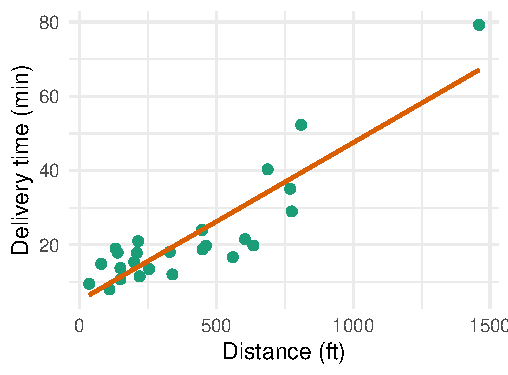
\includegraphics[width=\linewidth]{figures/delivery_raw_distance.pdf}}
            \mode<article>{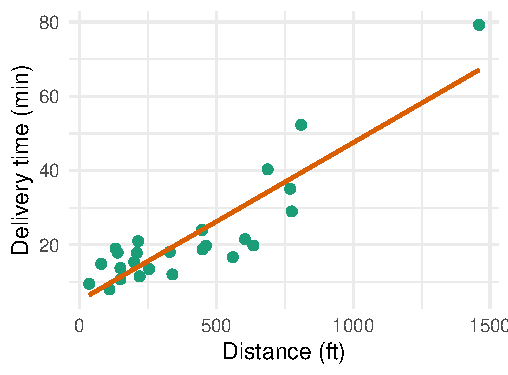
\includegraphics[width=0.8\linewidth]{figures/delivery_raw_distance.pdf}}
        \end{column}
    \end{columns}
\end{frame}


\begin{frame}{Constructing an Added-Variable Plot}
    Let $\bX_{(j)}$ be the design matrix with the column of $x_j$ removed (intercept kept).
    \begin{enumerate}
        \item Regress $y$ on $\bX_{(j)}$ and keep the residuals $e(y\mid\bX_{(j)})$.
        \item Regress $x_j$ on $\bX_{(j)}$ and keep the residuals $e(x_j\mid\bX_{(j)})$.
        \item Plot $e(y\mid\bX_{(j)})$ against $e(x_j\mid\bX_{(j)})$.
    \end{enumerate}
    \svspace{0.5em}
    Also called a partial regression plot.
\end{frame}


\begin{frame}{Residuals as Adjusted Variables}
    With $\mathbf{H}_{(j)}=\bX_{(j)}(\bX_{(j)}'\bX_{(j)})^{-1}\bX_{(j)}'$:
    \begin{align*}
        e(y\mid\bX_{(j)}) &= (\mathbf{I}-\mathbf{H}_{(j)})\by \\
        e(x_j\mid\bX_{(j)}) &= (\mathbf{I}-\mathbf{H}_{(j)})\bx_j
    \end{align*}
    \begin{itemize}
        \item The first is the part of $y$ not explained by the other regressors.
        \item The second is the part of $x_j$ not explained by the other regressors.
    \end{itemize}
\end{frame}


\begin{frame}{Delivery Time Data: Added-Variable Plot for Distance}
    \begin{columns}[T]
        \begin{column}{0.5\textwidth}
            \begin{itemize}
                \item Adjusted for cases, longer distances go with longer delivery times.
                \item The fitted line has slope $0.01438$, the coefficient $\hat\beta_2$ from the full model.
                \item Labelled points: 9 has the largest residual; 10 and 16 have the most extreme adjusted distance.
            \end{itemize}
        \end{column}
        \begin{column}{0.5\textwidth}
            \centering
            % Figure: delivery_av_distance.pdf (see extra-ss-delivery.R)
            \mode<presentation>{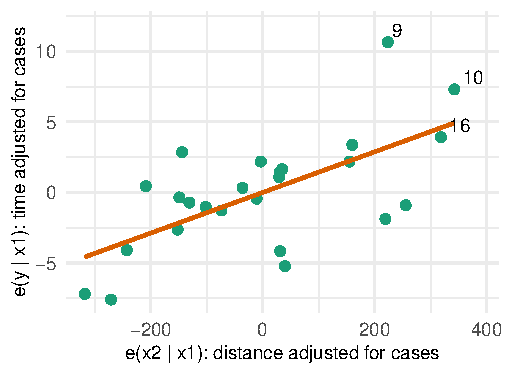
\includegraphics[width=\linewidth]{figures/delivery_av_distance.pdf}}
            \mode<article>{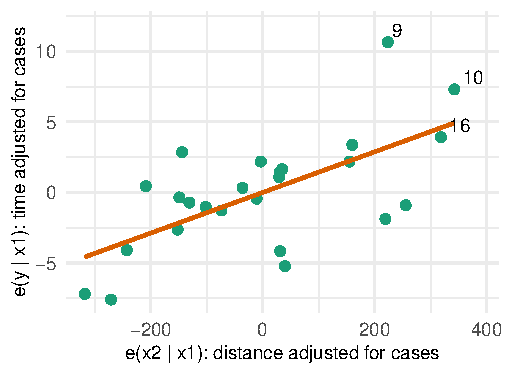
\includegraphics[width=0.8\linewidth]{figures/delivery_av_distance.pdf}}
        \end{column}
    \end{columns}
\end{frame}


\begin{frame}{Key Property: The Slope Is $\hat\beta_j$}
    The least-squares line through the added-variable plot has:
    \begin{itemize}
        \item Slope $\hat\beta_j$, the coefficient from the full model.
        \item Intercept $0$.
        \item Residuals equal to the full-model residuals $\mathbf{e}$.
    \end{itemize}
    \svspace{0.5em}
    The next two frames show why.
\end{frame}


\begin{frame}{Derivation, Step 1: Decompose $y$}
    The full-model fit separates $x_j$ from the other regressors:
    \[
    \by = \bX_{(j)}\hat{\bbeta}_{(j)} + \bx_j\hat\beta_j + \mathbf{e}
    \]
    Apply $\mathbf{I}-\mathbf{H}_{(j)}$. It annihilates $\bX_{(j)}$, and $(\mathbf{I}-\mathbf{H}_{(j)})\mathbf{e}=\mathbf{e}$ because $\mathbf{e}\perp\col(\bX)\supset\col(\bX_{(j)})$:
    \begin{align}
        e(y\mid\bX_{(j)}) = \hat\beta_j\,e(x_j\mid\bX_{(j)}) + \mathbf{e}
        \label{eq:av-decomp}
    \end{align}
\end{frame}


\begin{frame}{Derivation, Step 2: Slope and Residuals}
    Both adjusted variables have mean zero, so the line through the plot has no intercept. Its slope is
    \begin{align*}
        \frac{e(x_j\mid\bX_{(j)})'\,e(y\mid\bX_{(j)})}{e(x_j\mid\bX_{(j)})'\,e(x_j\mid\bX_{(j)})}
        = \hat\beta_j + \frac{e(x_j\mid\bX_{(j)})'\,\mathbf{e}}{e(x_j\mid\bX_{(j)})'\,e(x_j\mid\bX_{(j)})}
    \end{align*}
    The numerator of the last term is $\bx_j'(\mathbf{I}-\mathbf{H}_{(j)})\mathbf{e}=\bx_j'\mathbf{e}=0$. So the slope is $\hat\beta_j$ and, by \eqref{eq:av-decomp}, the residuals about the line are $\mathbf{e}$.
\end{frame}


\begin{frame}{Consequences}
    \begin{itemize}
        \item The plot has the same residuals, hence the same residual sum of squares, as the full model.
        \item The sum of squares explained by the line is $\hat\beta_j^{\,2}\sum_i e_i(x_j\mid\bX_{(j)})^2=\SSR(\beta_j\mid\text{others})$. Why: square both sides of \eqref{eq:av-decomp}; the cross term is $0$ because $e(x_j\mid\bX_{(j)})'\mathbf{e}=0$, so
        \[
        \underbrace{\textstyle\sum e(y\mid\bX_{(j)})^2}_{\SSRes(\text{without }x_j)} = \hat\beta_j^{\,2}\textstyle\sum e(x_j\mid\bX_{(j)})^2 + \underbrace{\mathbf{e}'\mathbf{e}}_{\SSRes(\FM)},
        \]
        and the difference of the two residual sums of squares is the extra sum of squares \eqref{eq:extra-ss-res}.
        \item Delivery data, distance: $0.014385^2\times813{,}838.7=168.40$.
        \item Outliers and influential points for $\hat\beta_j$ can be seen directly in the plot.
    \end{itemize}
\end{frame}


\begin{frame}{Delivery Time Data: Added-Variable Plot for Cases}
    \begin{columns}[T]
        \begin{column}{0.5\textwidth}
            \begin{itemize}
                \item Slope $1.616$, the full-model coefficient $\hat\beta_1$.
                \item The sum of squares due to the line is $951.66=\SSR(\beta_1\mid\beta_2,\beta_0)$.
                \item Point 22 has the most extreme adjusted number of cases.
                \item Point 9 again has the largest residual.
            \end{itemize}
        \end{column}
        \begin{column}{0.5\textwidth}
            \centering
            % Figure: delivery_av_cases.pdf (see extra-ss-delivery.R)
            \mode<presentation>{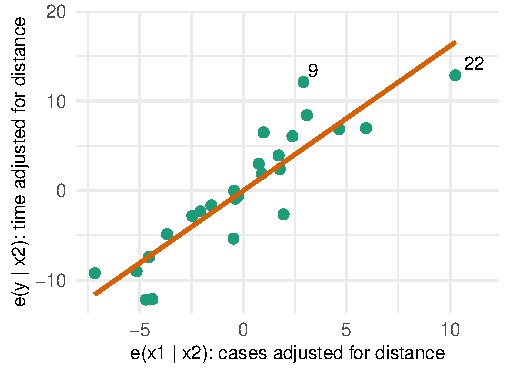
\includegraphics[width=\linewidth]{figures/delivery_av_cases.pdf}}
            \mode<article>{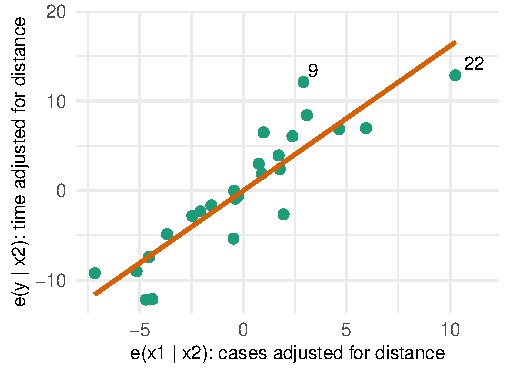
\includegraphics[width=0.8\linewidth]{figures/delivery_av_cases.pdf}}
        \end{column}
    \end{columns}
\end{frame}


\begin{frame}{Added-Variable Plots in R: \texttt{car::avPlots()}}
    \begin{center}
        % Figure: delivery_avplots_car.pdf (see extra-ss-delivery.R)
        \mode<presentation>{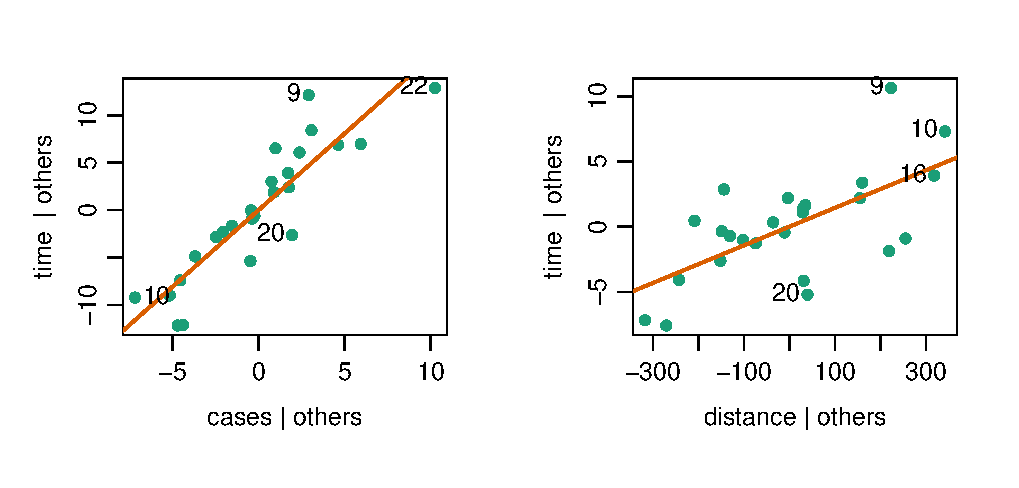
\includegraphics[width=0.75\linewidth]{figures/delivery_avplots_car.pdf}}
        \mode<article>{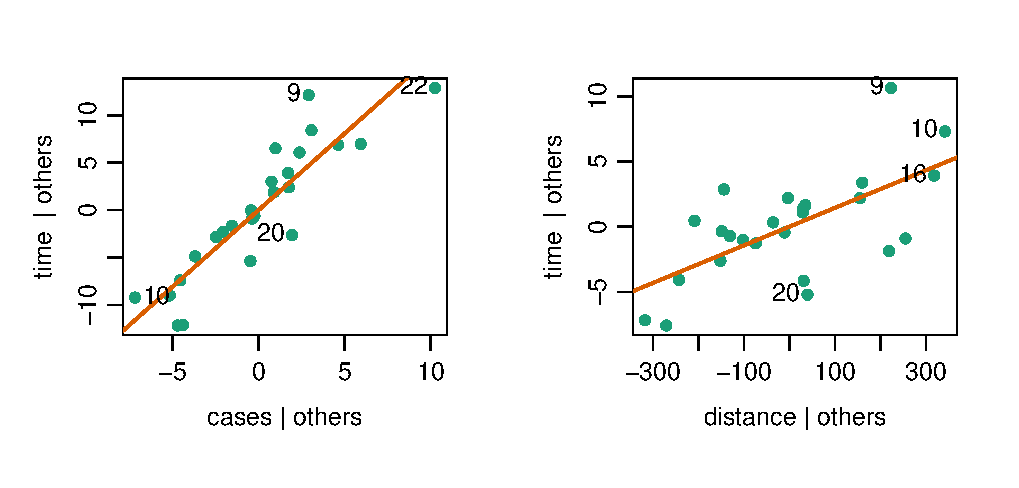
\includegraphics[width=0.9\linewidth]{figures/delivery_avplots_car.pdf}}
    \end{center}
    \begin{itemize}
        \item \texttt{car::avPlots(fit)} draws one panel per regressor, the same plots as the previous two slides.
        \item By default it labels the two largest residuals (9, 20) and the two most extreme points horizontally in each panel.
    \end{itemize}
\end{frame}


\begin{frame}{Squared Correlation in the Plot}
    The squared correlation between the two adjusted variables is
    \begin{align*}
        r^2 = \frac{\hat\beta_j^{\,2}\sum e(x_j\mid\bX_{(j)})^2}{\sum e(y\mid\bX_{(j)})^2}
        = \frac{\SSR(\beta_j\mid\text{others})}{\SSRes(\text{model without }x_j)}
    \end{align*}
    \begin{itemize}
        \item Distance: $168.40/402.13=0.419$, correlation $0.647$.
        \item Cases: $951.66/1185.39=0.803$, correlation $0.896$.
        \item This is the partial correlation of $y$ and $x_j$ given the other regressors; it returns in model selection.
    \end{itemize}
\end{frame}


\begin{frame}{Collinearity in the Plot}
    The horizontal spread of the plot is what is left of $x_j$ after the other regressors take their share:
    \[
    \sum_i e_i(x_j\mid\bX_{(j)})^2 = (1-R_j^2)\sum_i(x_{ij}-\bar x_j)^2,
    \qquad
    \Var(\hat\beta_j)=\frac{\sigma^2}{\sum_i e_i(x_j\mid\bX_{(j)})^2}
    \]
    \begin{itemize}
        \item $R_j^2$ is the $R^2$ from regressing $x_j$ on the other regressors.
        \item Delivery data: $\sum_i(x_{i2}-\bar x_2)^2=2{,}537{,}935$ for distance falls to $\sum_i e_i(x_2\mid x_1)^2=813{,}838.7$ after adjusting for cases, a fraction $0.321=1-0.824^2$, where $0.824=\Corr(x_1,x_2)$.
        \item $1/(1-R_j^2)$ is the variance inflation factor (VIF), covered next lecture; here $1/0.321=3.12$.
        \item Strong collinearity gives a narrow plot and an imprecise slope.
    \end{itemize}
\end{frame}


\begin{frame}{What to Look for in an Added-Variable Plot}
    \begin{itemize}
        \item Linearity: a straight band supports a linear term in $x_j$.
        \item Points far from the line: outliers after adjusting for the other regressors.
        \item Points extreme horizontally: potentially influential for $\hat\beta_j$.
        \item A narrow horizontal spread: collinearity between $x_j$ and the other regressors.
    \end{itemize}
\end{frame}


\begin{frame}{Question: A Point Far from the Line}
    \begin{itemize}
        \item A point lies far from the line in the added-variable plot but looks ordinary in the raw scatterplot of $y$ against $x_j$.
        \item What does this tell you?
    \end{itemize}
    % Answer:
    % - Given the other regressors, the observation's response is unusual, an outlier that the raw plot hides because the other regressors explain much of the raw variation.
    % - It deserves a closer look in the residual analysis, since it inflates SSRes and can shift the fit.
\end{frame}


\begin{frame}{Partial Residual Plot: A Companion}
    \begin{columns}[T]
        \begin{column}{0.5\textwidth}
            \begin{itemize}
                \item Plot $e_i+\hat\beta_j x_{ij}$ against $x_{ij}$.
                \item Slope is $\hat\beta_j$, as in the added-variable plot.
                \item The horizontal axis keeps the original scale of $x_j$.
                \item Curvature in the effect of $x_j$ is easier to see here.
            \end{itemize}
        \end{column}
        \begin{column}{0.5\textwidth}
            \centering
            % Figure: delivery_pr_distance.pdf (see extra-ss-delivery.R)
            \mode<presentation>{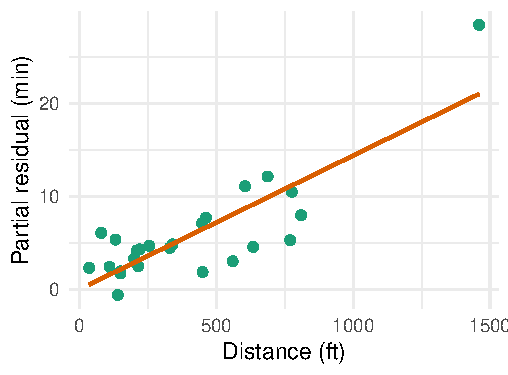
\includegraphics[width=\linewidth]{figures/delivery_pr_distance.pdf}}
            \mode<article>{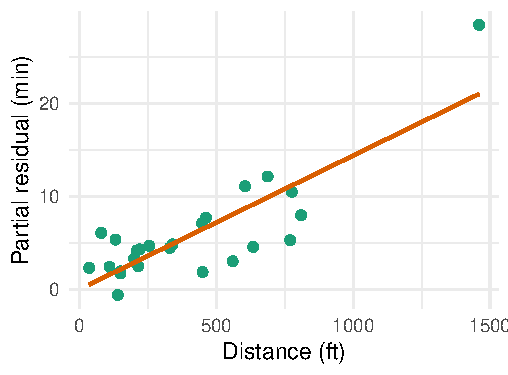
\includegraphics[width=0.8\linewidth]{figures/delivery_pr_distance.pdf}}
        \end{column}
    \end{columns}
\end{frame}


\begin{frame}{Limits of Added-Variable Plots}
    \begin{itemize}
        \item They show the partial effect of one regressor under a linear model for the others.
        \item They are not the best tool for deciding which transformation of $x_j$ is needed; use a partial residual plot for that.
        \item A relationship between $x_j$ and the other regressors that is not linear can distort the picture.
        \item They are a diagnostic, not a test: the $F$-test of $\beta_j$ remains the formal tool.
    \end{itemize}
\end{frame}


\section{Summary}


\begin{frame}{Summary of Tests}
    \begin{center}
        \small
        \begin{tabular}{llcl}
            \toprule
            Test & Hypothesis & $q$ & Reduced model \\
            \midrule
            Overall & $\beta_1=\cdots=\beta_k=0$ & $k$ & Intercept only \\
            Individual & $\beta_j=0$ & 1 & Drop $x_j$ \\
            Subset (partial $F$) & $\bbeta_{(2)}=\mathbf{0}$ & $q$ & Drop $\bX_2$ \\
            General linear & $\mathbf{T}\bbeta=\mathbf{0}$ & $q$ & Impose restrictions \\
            \bottomrule
        \end{tabular}
    \end{center}
    All use $F_0=\dfrac{[\SSRes(\RM)-\SSRes(\FM)]/q}{\SSRes(\FM)/(n-p)}\sim F_{q,\,n-p}$.
\end{frame}


\begin{frame}{Key Takeaways}
    \begin{itemize}
        \item A full-versus-reduced comparison tests any group of coefficients through one $F$ statistic.
        \item The extra sum of squares is the drop in $\SSRes$, with one degree of freedom per added parameter.
        \item Individual $t$-tests can all be insignificant while a group is highly significant.
        \item Sequential sums of squares depend on order and add up; partial sums of squares adjust for everything else and do not.
        \item An added-variable plot shows $\hat\beta_j$, the full-model residuals and $\SSR(\beta_j\mid\text{others})$ in one picture.
    \end{itemize}
\end{frame}
